\section{CAT Constraint Acquisition}

\begin{frame}
\frametitle{Based on previous work with}
\begin{textblock*}{6cm}(9cm,1cm)
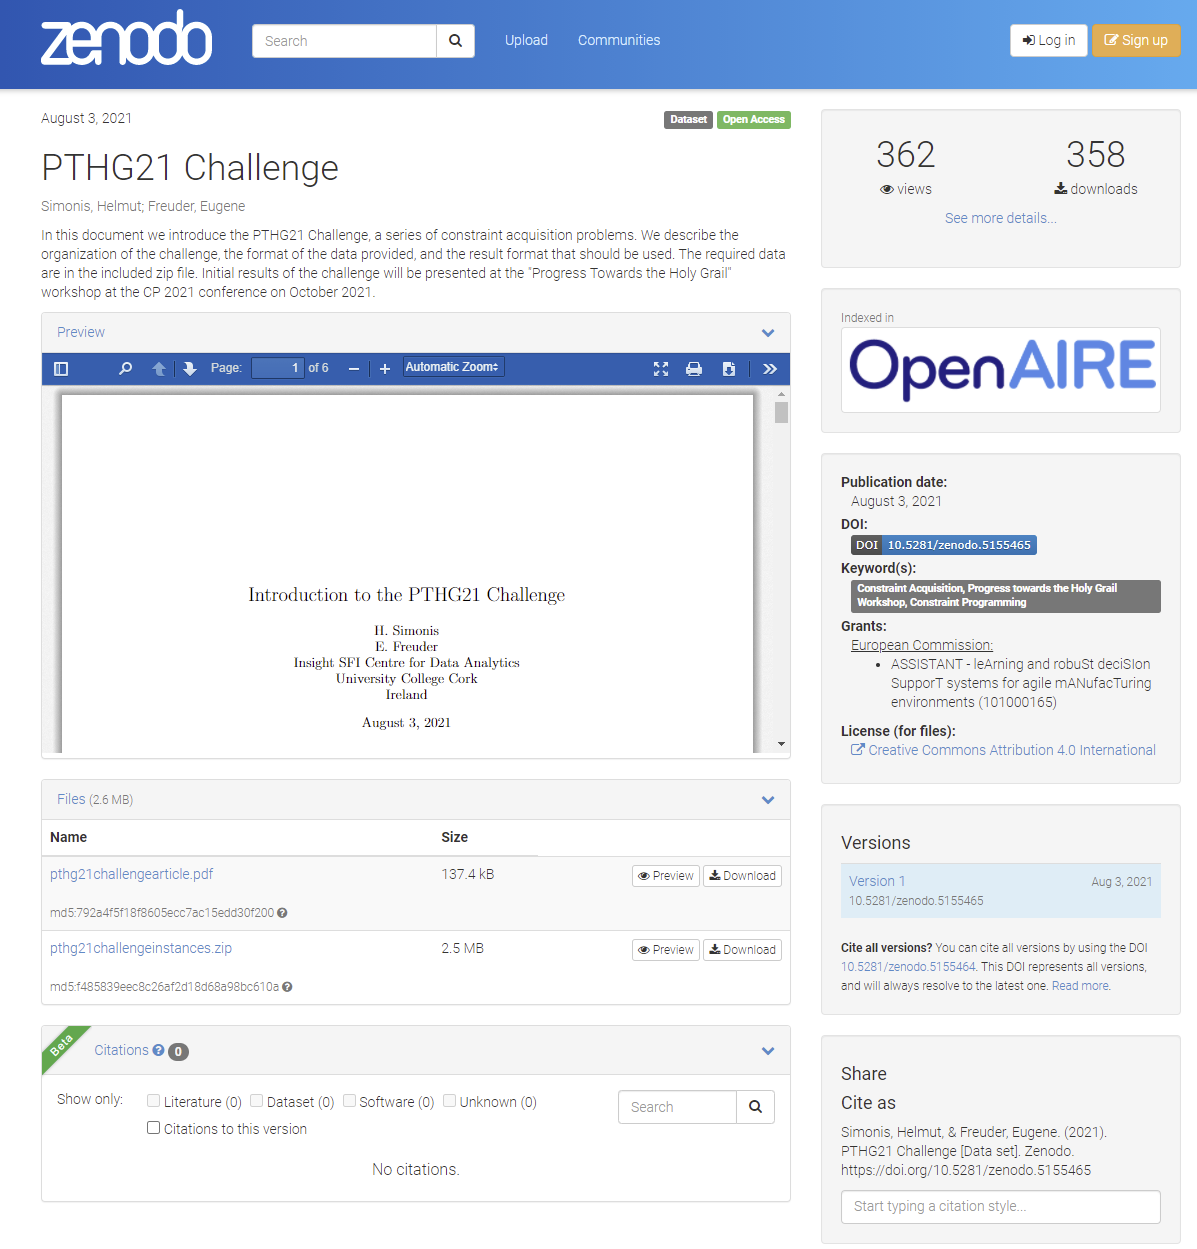
\includegraphics[width=6cm]{imagescat/zenodo.png}
\end{textblock*}

\begin{itemize}
\item N. Beldiceanu, IMT Atlantique
\item M. Carlsson, SICS
\end{itemize}
\vspace{2cm}
PTHG21 Challenge co-organized with E. Freuder
\end{frame}

\subsection{Introduction}

\begin{frame}
\frametitle{Industrial Problem}
\begin{itemize}
\item Industry
\item Optimization Projects are hard to manage
\item Skilled experts are not easily found
\item Communication between domain experts and programmers key
\item Easy to miss key constraint during design 
\end{itemize}
\end{frame}

\begin{frame}
\frametitle{Research Challenge}
\begin{itemize}
\item How can we make optimization more accessible?
\item Lower barriers to entry
\item or, make existing experts more productive
\item Bridge gap between application domain and abstract optimization concepts
\end{itemize}
\end{frame}

\begin{frame}
\frametitle{Take-Away Points}
\begin{itemize}
\item Constraint Acquisition provides a way to learn constraint model from data
\item Questions about use cases
\item Transferable, executable models
\item Common benchmark set: PTHG21 Challenge
\item CAT System shows feasibility of approach
\end{itemize}
\end{frame}

\begin{frame}
\frametitle{Background}
\begin{itemize}
\item ASSISTANT project (EU H2020, ICT-38 project, \url{https://assistant-project.eu/})
\item Constraint Acquisition part of WP 4
\item Making Constraint Acquisition relevant in real world, scheduling setting
\item Based on case studies from Siemens Energy and Atlas Copco
\end{itemize}
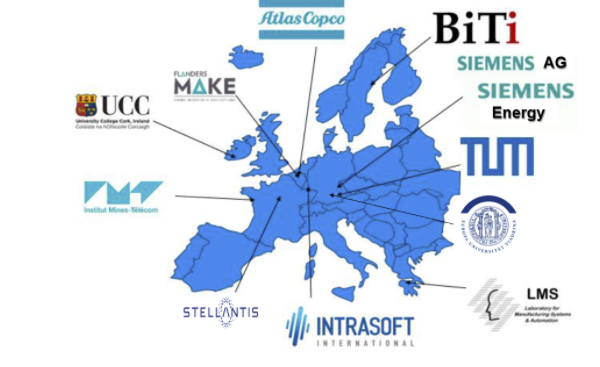
\includegraphics[width=5cm]{imagescat/assistantpartners}
\end{frame}

\subsection{Solution Approach}
\begin{frame}
\frametitle{Constraint Acquisition - What is it?}
\begin{itemize}
\item Learn Constraint Models from data
\begin{itemize}
\item Given positive and negative examples ("Passive")
\item Asking questions to user ("Active")
\end{itemize}
\item Useful to
\begin{itemize}
\item Understand problem
\item Classify new examples as solutions or non-solutions
\item Use generated model to find solutions 
\end{itemize}
\end{itemize}
\end{frame}

% \begin{frame}
% \frametitle{Literature}
% \begin{itemize}
% \item Christian Bessiere, Frédéric Koriche, Nadjib Lazaar, Barry O'Sullivan:
% Constraint acquisition. Artif. Intell. 244: 315-342 (2017)
% \item Remi Coletta, Christian Bessière, Barry O'Sullivan, Eugene C. Freuder, Sarah O'Connell, Joël Quinqueton:
% Semi-automatic Modeling by Constraint Acquisition. CP 2003: 812-816
% \item Christian Bessiere, Remi Coletta, Frédéric Koriche, Barry O'Sullivan:
% Acquiring Constraint Networks Using a SAT-based Version Space Algorithm. AAAI 2006: 1565-1568
% \item Mohit Kumar, Stefano Teso, Luc De Raedt:
% Acquiring Integer Programs from Data. IJCAI 2019: 1130-1136
% \item Nicolas Beldiceanu, Helmut Simonis:
% A Model Seeker: Extracting Global Constraint Models from Positive Examples. CP 2012: 141-157

% \end{itemize}
% \end{frame}

% \begin{frame}
% \frametitle{State of the Art Discussion}
% \begin{itemize}
% \item Many different approaches
% \item Not based on a common use case
% \item Comparison of results difficult
% \item PTHG21 Challenge tried to shape discussion
% \end{itemize}
% \end{frame}

% \begin{frame}<1>[label=zooms]
  \frametitle{Example: Sudoku}
  \framezoom<1><2>(0cm,0cm)(4.2cm,2.7cm)
  \framezoom<1><3>(10.3cm,0cm)(4.7cm,2.5cm)
  \framezoom<1><4>(2.6cm,2.8cm)(10.2cm,3.9cm)
  \scalebox{0.4}{
  \begin{tikzpicture}[xscale=5,yscale=3,
  inputdata/.style={fill=insight-burntorange!10,draw=black,rounded corners},
program/.style={fill=insight-lime!20,draw=black!30},
documents/.style={fill=insight-royalblue!20,draw=black!30,rounded corners,drop shadow},
positive/.style={fill=insight-aqua!20,draw=black!30,rounded corners,drop shadow},
negative/.style={fill=insight-burntorange!20,draw=black!30,rounded corners,drop shadow},
test/.style={fill=insight-plum!20,draw=black!30,rounded corners,drop shadow},
extrasolution/.style={fill=insight-yellow!20,draw=black!30,rounded corners,drop shadow},
document/.style={fill=insight-royalblue!20,draw=black,rounded corners}]

    \draw[draw,rounded corners] (0.7,1.5) rectangle (1.3,3.5);
    \node[below] at(1,1.5) {\LARGE Instance 1};
    
    \draw[draw,rounded corners] (1.4,1.5) rectangle (2.7,3.5);
    \node[below] at(2,1.5) {\LARGE Instance 2};
    
    \node[positive,label={90:Solution}] at (1,3)
      {\scriptsize  \begin{tabular}{cccc}1&3&2&4\\
2&4&1&3\\
3&1&4&2\\
4&2&3&1\\
\end{tabular}};

    \node[negative,label={90:Nonsolution}] at (1,2)         
{\scriptsize \begin{tabular}{cccc}
2&4&3&3\\
1&3&4&2\\
4&2&3&1\\
3&1&2&4\\
\end{tabular}};

    \node[positive] at (2,3)
{\tiny \begin{tabular}{*{9}{c}}
9&5&7&6&4&8&3&2&1\\
4&8&3&1&5&2&6&9&7\\
1&6&2&9&7&3&5&8&4\\
5&2&1&8&3&6&4&7&9\\
3&9&6&4&1&7&2&5&8\\
7&4&8&5&2&9&1&3&6\\
6&3&9&2&8&4&7&1&5\\
8&7&5&3&6&1&9&4&2\\
2&1&4&7&9&5&8&6&3\\
\end{tabular}};

    \node[negative] at (2,2)
{\tiny
\begin{tabular}{*{9}{c}}
7&1&3&6&9&2&8&5&4\\
8&8&2&5&7&4&1&3&9\\
5&5&4&1&8&3&7&2&6\\
3&3&9&4&6&1&5&8&7\\
6&7&1&8&2&5&9&4&3\\
5&8&5&9&3&7&2&6&1\\
8&3&6&2&5&8&5&7&5\\
2&5&7&3&4&9&6&1&8\\
1&4&8&7&5&7&3&9&2\\
\end{tabular}};

\node[program] (ca) at (3.5,2.5) {\Huge \shortstack{Constraint\\Acquisition}};
\node[program] (classify) at (3.5,1.5) {\Huge \shortstack{Classify\\Tests}};

\node[document,label={90:\LARGE Model}] (model) at (4.6,2.5) {\Huge\shortstack[l]{Each Row:\\ alldifferent\\Each Column:\\ alldifferent\\Each Block:\\ alldifferent}};
\node[program] (solver) at (5.5,2.5) {\Huge Solver};

\node[extrasolution,label={90:\LARGE Extra Solutions}] (extra) at (7,2.5)
     {\tiny \begin{tabular}{*{16}{c}}
16& 15& 14& 13& 12& 11& 10& 9& 8& 7& 6& 5& 4& 3& 2& 1\\
12& 11& 10& 9& 16& 15& 14& 13& 4& 3& 2& 1& 8& 7& 6& 5\\
8& 7& 6& 5& 4& 3& 2& 1& 16& 15& 14& 13& 12& 11& 10& 9\\
4& 3& 2& 1& 8& 7& 6& 5& 12& 11& 10& 9& 16& 15& 14& 13\\
15& 16& 13& 14& 11& 12& 9& 10& 7& 8& 5& 6& 3& 4& 1& 2\\
11& 12& 9& 10& 15& 16& 13& 14& 3& 4& 1& 2& 7& 8& 5& 6\\
7& 8& 5& 6& 3& 4& 1& 2& 15& 16& 13& 14& 11& 12& 9& 10\\
3& 4& 1& 2& 7& 8& 5& 6& 11& 12& 9& 10& 15& 16& 13& 14\\
14& 13& 16& 15& 10& 9& 12& 11& 6& 5& 8& 7& 2& 1& 4& 3\\
10& 9& 12& 11& 14& 13& 16& 15& 2& 1& 4& 3& 6& 5& 8& 7\\
6& 5& 8& 7& 2& 1& 4& 3& 14& 13& 16& 15& 10& 9& 12& 11\\
2& 1& 4& 3& 6& 5& 8& 7& 10& 9& 12& 11& 14& 13& 16& 15\\
13& 14& 15& 16& 9& 10& 11& 12& 5& 6& 7& 8& 1& 2& 3& 4\\
9& 10& 11& 12& 13& 14& 15& 16& 1& 2& 3& 4& 5& 6& 7& 8\\
5& 6& 7& 8& 1& 2& 3& 4& 13& 14& 15& 16& 9& 10& 11& 12\\
1& 2& 3& 4& 5& 6& 7& 8& 9& 10& 11& 12& 13& 14& 15& 16\\
\end{tabular}};


\node[below,test] (test2) at (2.5,0)
{\tiny
\begin{tabular}{cccc}
1&4&2&3\\
2&3&4&1\\
4&1&3&2\\
3&2&1&4\\
\end{tabular}}; 

    \node[below,test] (test3) at (3.5,0)
{\tiny
\begin{tabular}{*{9}{c}}
3&9&1&5&6&6&7&4&2\\
6&2&8&3&7&9&1&5&6\\
5&7&1&2&1&4&9&3&8\\
8&3&9&4&6&2&4&7&5\\
7&1&4&8&5&3&2&6&9\\
2&5&6&9&4&7&3&8&1\\
6&8&2&7&3&5&6&1&4\\
1&4&3&6&2&8&5&9&7\\
7&7&5&4&9&1&8&2&3\\
\end{tabular}};

    \node[below,test,label={270:Unseen Size}] (test4) at (5.5,0)
{\tiny
\begin{tabular}{*{16}{c}}
8&13&12&4&14&16&3&9&7&1&6&11&10&5&15&2\\
10&7&1&5&12&2&13&6&8&9&4&9&3&14&2&11\\
9&14&15&3&1&11&5&8&13&10&2&16&6&7&12&4\\
11&16&6&2&10&15&3&7&3&1&12&5&6&13&8&9\\
5&11&8&6&13&8&12&7&1&3&16&2&14&15&9&10\\
16&12&9&14&2&7&1&10&15&5&11&9&13&6&4&8\\
15&5&4&1&9&3&6&16&14&8&10&13&7&2&11&12\\
2&10&13&7&11&3&15&14&12&6&7&4&3&1&3&5\\
14&1&12&8&16&13&14&5&9&15&3&7&8&9&13&6\\
3&8&9&7&6&13&10&12&4&11&1&14&14&16&5&15\\
6&15&11&13&7&1&9&3&16&12&5&8&2&8&10&14\\
5&4&5&16&15&12&8&11&6&2&13&10&9&3&1&7\\
13&6&16&11&10&9&2&15&5&7&8&12&4&10&13&1\\
5&9&7&8&4&13&11&1&2&13&14&3&15&12&6&16\\
1&2&10&12&8&14&16&13&11&4&12&6&5&9&7&3\\
4&3&14&15&5&6&2&13&10&16&9&1&11&8&2&8\\
\end{tabular}};

\draw[draw,rounded corners] (2,0.3) rectangle(7,-1.8);
\node[below] at (4,-1.8){\LARGE Tests}; 

\draw[->] (2.7,2.5) -- (ca);
  \draw[->] (ca) -- (model);
  \draw[->] (ca) -- (classify);
    \draw[->] (model) -- (solver);
    \draw[->] (solver) -- (extra);
  \draw[<->] (classify) -- node[above left,insight-aqua] {\LARGE sol} (test2);
  \draw[<->] (classify) -- node[left,insight-burntorange] {\LARGE nonsol} (test3);
  \draw[<->] (classify) -- node[above right,insight-burntorange] {\LARGE nonsol} (test4);

  \end{tikzpicture}
  }

\end{frame}



% \begin{frame}[fragile]
% \frametitle{Generic Sudoku Model (MiniZinc, generated by CAT)}
% \lstinputlisting[language=Mzn]{type06.mzn}
% \end{frame}

% \begin{frame}
\frametitle{Generic Sudoku Description}
\begin{block}{Generated by CAT}
Given an integer parameter \emph{size}, 
find an assignment for a matrix \emph{x} with \emph{nsquare(size)} rows and \emph{nsquare(size)} columns, where each element ranges between \emph{1} and \emph{nsquare(size)},

\noindent such that
\begin{description}
\item[1] the elements of each row of \emph{x} are pairwise different (\emph{permutation} constraint).


\item[2] the elements of each column of \emph{x} are pairwise different (\emph{permutation} constraint).


\item[3] the elements of each major block (of size \emph{size}$\times$\emph{size}) of \emph{x} are pairwise different (\emph{permutation} constraint).


\end{description}
\end{block}
\end{frame}


% \begin{frame}
% \frametitle{Use Case}
% \begin{itemize}
% \item Get past solutions and non-solutions from end-user
% \item Generate generic model of problem
% \item Allows only limited interaction with end-user
% \item Use generated model to solve future, unseen instances
% \item Given all background (input) data that would be available to current scheduler
% \item Aim: demonstrate feasibility of Constraint Acquisition as an end-to-end tool chain
% \end{itemize}
% \end{frame}

\begin{frame}
\frametitle{Intended Use Case}
\scalebox{0.8}{
\begin{tikzpicture}[xscale=2.5,yscale=2,
inputdata/.style={fill=insight-burntorange!10,draw=black,rounded corners},
program/.style={fill=insight-lime!20,draw=black!30},
documents/.style={fill=insight-royalblue!20,draw=black!30,rounded corners,drop shadow},
document/.style={fill=insight-royalblue!20,draw=black,rounded corners}]
\draw[inputdata] (0.25,1.5) rectangle (1.35,4.5);
\node[documents] (input) at (0.75,4) {\shortstack{Input\\Data}};
\node[documents] (solutions) at (0.75,3) {Solutions};
\node[documents] (nonsolutions) at (0.75,2) {NonSolutions};
\node[below] at (0.75,1.5) {\tiny Instances, multiple sizes};
\node[program] (ca) at (2,3) {\shortstack{Constraint\\Acquisition}};
\node[document] (model) at (3,3) {\shortstack{Generic\\Model}};
\node[documents] (unseen) at (4,4) {\shortstack{Unseen\\Input}};
\node[program] (solver) at (4,3) {Solver};
\node[documents] (solution) at (5,3) {Solution};
\node[] (user) at (2.5,1.5) {User};
\draw[->] (input) -- (ca);
\draw[->] (solutions) -- (ca);
\draw[->] (nonsolutions) -- (ca);
\draw[->] (ca) -- (model);
\draw[->] (model) -- (solver);
\draw[->] (unseen) -- (solver);
\draw[->] (solver) -- (solution);
\draw[->,dotted] (user) -- (ca);
\draw[->,dotted] (user) -- (model);
\end{tikzpicture}
}
\begin{itemize}
\item Aim: demonstrate feasibility of Constraint Acquisition as an end-to-end tool chain
\end{itemize}

\end{frame}


\begin{frame}
\frametitle{Properties}
\begin{itemize}
\item Generated model must be transferable to new data
\item Problem size varies from day to day
\item Some variables of model may not be exposed in solution provided
\begin{itemize}
\item Auxiliary variables not interesting to user
\item Individual cost elements
\end{itemize}
\item Constraints are there for a reason
\begin{itemize}
\item Due to structure of problem (think: Sudoku)
\item Due to input data (think: Graph Colouring)
\end{itemize}
\end{itemize}
\end{frame}

\begin{frame}
\frametitle{PTHG21 Challenge}
\scalebox{0.9}{
\begin{tikzpicture}[xscale=2.8,yscale=2.5,
participant/.style={fill=insight-burntorange!10,draw=black,rounded corners},
program/.style={fill=insight-lime!20,draw=black!30},
internaldocuments/.style={fill=insight-royalblue!10,draw=black!30,rounded corners,drop shadow},
documents/.style={fill=insight-royalblue!20,draw=black!30,rounded corners,drop shadow},
document/.style={fill=insight-royalblue!20,draw=black,rounded corners},
score/.style={fill=insight-yellow!20,draw=black!30}]
\draw[participant] (2.5,1.5) rectangle (4.5,3.5);
\node[below] at (3,1.5) {Participant};
\node[program] (generator) at (1,3) {\shortstack{Dataset\\Generator}};
\node[documents] (instances) at (2,3) {\shortstack[l]{Input Data\\Template\\Solutions\\NonSolutions\\Tests}};
\node[below] at (2,2.5) {\scriptsize Multiple Sizes};
\node[program] (checker) at (3,4) {Checker};
\node[internaldocuments] (refsol) at (4,4) {\shortstack{Intended\\Classification}};
\node[program] (cat) at (3,3) {\shortstack{User\\Acquisition\\Tool}};
\node[documents] (testresult) at (4,3) {\shortstack{Test\\Classification}};
\node[documents] (extrasol) at (4,2) {\shortstack{Extra\\Solutions}};
\node[program] (testeval) at (5,3) {\shortstack{Test\\Evaluation}};
\node[program] (checker2) at (5,2) {Checker};
\node[score] (score) at (6,2.5) {Score};
\draw[->] (generator) -- (instances);
\draw[->] (instances) -- (cat);
\draw[->] (instances) -- (checker);
\draw[->] (checker) -- (refsol);
\draw[->] (cat) -- (testresult);
\draw[->] (cat) -- (extrasol);
\draw[->] (testresult) -- (testeval);
\draw[->] (refsol) -- (testeval);
\draw[->] (testeval) -- (score);
\draw[->] (extrasol) -- (checker2);
\draw[->] (checker2) -- (score);
\end{tikzpicture}
}
\end{frame}


%\begin{frame}<1>[label=zooms]
  \frametitle{Example: Sudoku}
  \framezoom<1><2>(0cm,0cm)(4.2cm,2.7cm)
  \framezoom<1><3>(10.3cm,0cm)(4.7cm,2.5cm)
  \framezoom<1><4>(2.6cm,2.8cm)(10.2cm,3.9cm)
  \scalebox{0.4}{
  \begin{tikzpicture}[xscale=5,yscale=3,
  inputdata/.style={fill=insight-burntorange!10,draw=black,rounded corners},
program/.style={fill=insight-lime!20,draw=black!30},
documents/.style={fill=insight-royalblue!20,draw=black!30,rounded corners,drop shadow},
positive/.style={fill=insight-aqua!20,draw=black!30,rounded corners,drop shadow},
negative/.style={fill=insight-burntorange!20,draw=black!30,rounded corners,drop shadow},
test/.style={fill=insight-plum!20,draw=black!30,rounded corners,drop shadow},
extrasolution/.style={fill=insight-yellow!20,draw=black!30,rounded corners,drop shadow},
document/.style={fill=insight-royalblue!20,draw=black,rounded corners}]

    \draw[draw,rounded corners] (0.7,1.5) rectangle (1.3,3.5);
    \node[below] at(1,1.5) {\LARGE Instance 1};
    
    \draw[draw,rounded corners] (1.4,1.5) rectangle (2.7,3.5);
    \node[below] at(2,1.5) {\LARGE Instance 2};
    
    \node[positive,label={90:Solution}] at (1,3)
      {\scriptsize  \begin{tabular}{cccc}1&3&2&4\\
2&4&1&3\\
3&1&4&2\\
4&2&3&1\\
\end{tabular}};

    \node[negative,label={90:Nonsolution}] at (1,2)         
{\scriptsize \begin{tabular}{cccc}
2&4&3&3\\
1&3&4&2\\
4&2&3&1\\
3&1&2&4\\
\end{tabular}};

    \node[positive] at (2,3)
{\tiny \begin{tabular}{*{9}{c}}
9&5&7&6&4&8&3&2&1\\
4&8&3&1&5&2&6&9&7\\
1&6&2&9&7&3&5&8&4\\
5&2&1&8&3&6&4&7&9\\
3&9&6&4&1&7&2&5&8\\
7&4&8&5&2&9&1&3&6\\
6&3&9&2&8&4&7&1&5\\
8&7&5&3&6&1&9&4&2\\
2&1&4&7&9&5&8&6&3\\
\end{tabular}};

    \node[negative] at (2,2)
{\tiny
\begin{tabular}{*{9}{c}}
7&1&3&6&9&2&8&5&4\\
8&8&2&5&7&4&1&3&9\\
5&5&4&1&8&3&7&2&6\\
3&3&9&4&6&1&5&8&7\\
6&7&1&8&2&5&9&4&3\\
5&8&5&9&3&7&2&6&1\\
8&3&6&2&5&8&5&7&5\\
2&5&7&3&4&9&6&1&8\\
1&4&8&7&5&7&3&9&2\\
\end{tabular}};

\node[program] (ca) at (3.5,2.5) {\Huge \shortstack{Constraint\\Acquisition}};
\node[program] (classify) at (3.5,1.5) {\Huge \shortstack{Classify\\Tests}};

\node[document,label={90:\LARGE Model}] (model) at (4.6,2.5) {\Huge\shortstack[l]{Each Row:\\ alldifferent\\Each Column:\\ alldifferent\\Each Block:\\ alldifferent}};
\node[program] (solver) at (5.5,2.5) {\Huge Solver};

\node[extrasolution,label={90:\LARGE Extra Solutions}] (extra) at (7,2.5)
     {\tiny \begin{tabular}{*{16}{c}}
16& 15& 14& 13& 12& 11& 10& 9& 8& 7& 6& 5& 4& 3& 2& 1\\
12& 11& 10& 9& 16& 15& 14& 13& 4& 3& 2& 1& 8& 7& 6& 5\\
8& 7& 6& 5& 4& 3& 2& 1& 16& 15& 14& 13& 12& 11& 10& 9\\
4& 3& 2& 1& 8& 7& 6& 5& 12& 11& 10& 9& 16& 15& 14& 13\\
15& 16& 13& 14& 11& 12& 9& 10& 7& 8& 5& 6& 3& 4& 1& 2\\
11& 12& 9& 10& 15& 16& 13& 14& 3& 4& 1& 2& 7& 8& 5& 6\\
7& 8& 5& 6& 3& 4& 1& 2& 15& 16& 13& 14& 11& 12& 9& 10\\
3& 4& 1& 2& 7& 8& 5& 6& 11& 12& 9& 10& 15& 16& 13& 14\\
14& 13& 16& 15& 10& 9& 12& 11& 6& 5& 8& 7& 2& 1& 4& 3\\
10& 9& 12& 11& 14& 13& 16& 15& 2& 1& 4& 3& 6& 5& 8& 7\\
6& 5& 8& 7& 2& 1& 4& 3& 14& 13& 16& 15& 10& 9& 12& 11\\
2& 1& 4& 3& 6& 5& 8& 7& 10& 9& 12& 11& 14& 13& 16& 15\\
13& 14& 15& 16& 9& 10& 11& 12& 5& 6& 7& 8& 1& 2& 3& 4\\
9& 10& 11& 12& 13& 14& 15& 16& 1& 2& 3& 4& 5& 6& 7& 8\\
5& 6& 7& 8& 1& 2& 3& 4& 13& 14& 15& 16& 9& 10& 11& 12\\
1& 2& 3& 4& 5& 6& 7& 8& 9& 10& 11& 12& 13& 14& 15& 16\\
\end{tabular}};


\node[below,test] (test2) at (2.5,0)
{\tiny
\begin{tabular}{cccc}
1&4&2&3\\
2&3&4&1\\
4&1&3&2\\
3&2&1&4\\
\end{tabular}}; 

    \node[below,test] (test3) at (3.5,0)
{\tiny
\begin{tabular}{*{9}{c}}
3&9&1&5&6&6&7&4&2\\
6&2&8&3&7&9&1&5&6\\
5&7&1&2&1&4&9&3&8\\
8&3&9&4&6&2&4&7&5\\
7&1&4&8&5&3&2&6&9\\
2&5&6&9&4&7&3&8&1\\
6&8&2&7&3&5&6&1&4\\
1&4&3&6&2&8&5&9&7\\
7&7&5&4&9&1&8&2&3\\
\end{tabular}};

    \node[below,test,label={270:Unseen Size}] (test4) at (5.5,0)
{\tiny
\begin{tabular}{*{16}{c}}
8&13&12&4&14&16&3&9&7&1&6&11&10&5&15&2\\
10&7&1&5&12&2&13&6&8&9&4&9&3&14&2&11\\
9&14&15&3&1&11&5&8&13&10&2&16&6&7&12&4\\
11&16&6&2&10&15&3&7&3&1&12&5&6&13&8&9\\
5&11&8&6&13&8&12&7&1&3&16&2&14&15&9&10\\
16&12&9&14&2&7&1&10&15&5&11&9&13&6&4&8\\
15&5&4&1&9&3&6&16&14&8&10&13&7&2&11&12\\
2&10&13&7&11&3&15&14&12&6&7&4&3&1&3&5\\
14&1&12&8&16&13&14&5&9&15&3&7&8&9&13&6\\
3&8&9&7&6&13&10&12&4&11&1&14&14&16&5&15\\
6&15&11&13&7&1&9&3&16&12&5&8&2&8&10&14\\
5&4&5&16&15&12&8&11&6&2&13&10&9&3&1&7\\
13&6&16&11&10&9&2&15&5&7&8&12&4&10&13&1\\
5&9&7&8&4&13&11&1&2&13&14&3&15&12&6&16\\
1&2&10&12&8&14&16&13&11&4&12&6&5&9&7&3\\
4&3&14&15&5&6&2&13&10&16&9&1&11&8&2&8\\
\end{tabular}};

\draw[draw,rounded corners] (2,0.3) rectangle(7,-1.8);
\node[below] at (4,-1.8){\LARGE Tests}; 

\draw[->] (2.7,2.5) -- (ca);
  \draw[->] (ca) -- (model);
  \draw[->] (ca) -- (classify);
    \draw[->] (model) -- (solver);
    \draw[->] (solver) -- (extra);
  \draw[<->] (classify) -- node[above left,insight-aqua] {\LARGE sol} (test2);
  \draw[<->] (classify) -- node[left,insight-burntorange] {\LARGE nonsol} (test3);
  \draw[<->] (classify) -- node[above right,insight-burntorange] {\LARGE nonsol} (test4);

  \end{tikzpicture}
  }

\end{frame}




\begin{frame}
\frametitle{Challenge Problems (Set 1)}
\scalebox{0.8}{
\begin{tabular}{*{4}{r}} \toprule
Type & Problem & Source & Features \\ \midrule
1 & Graph Coloring & ALICE, CHIP & graph as data, optimization\\
2 & N-Queens & CSPlib 054& \\
3 & Warehouse Location & CSPlib 034& cost matrix/vector as data, implicit cost variables\\
4 & Golomb Ruler & CSPlib 006& implicit decision variables, optimization\\
5 & Sudoku  & Pre-assignment& pre-assignment as data, single solution\\
6 & Sudoku & No pre-assignment& many solutions\\
7 & Schur's Lemma & CSPlib 015 & non-standard variable pattern, ternary constraint\\
8 & All Interval & CSPlib 007& auxiliary variables\\
10 & Magic Squares & CSPlib 019& implicit formula\\
11 & Orthogonal Latin Squares & Euler & constraint on tuples\\
12 & BIBD & CSPlib 028& 3 parameters, implicit formulas, symmetry breaking\\
13 & Costas Array & CSPlib 076& auxiliary variables, constraint on tuples\\
14 & N-Queens variant& fairy chess piece & non-traditional attack\\
15 & N-Queens variant& \\
16 & N-Queens variant& \\
\bottomrule
\end{tabular}
}
\end{frame}



\begin{frame}
\frametitle{The CAT System}
\begin{itemize}
\item Find global constraint models comparable to hand-built solutions
\item Assumption: All needed information is either given as data or in regular structure
\item Transferable, executable models for class of instances
\item Built bottom up, based on test cases
\item Should extend to more complex cases \\in more narrow application domain
\end{itemize}
\end{frame}

\begin{frame}<1>[label=catarchitecture]
\frametitle{The CAT System Architecture}
%\framezoom<1><2>[border](0cm,0cm)(6cm,3.7cm)
%\framezoom<1><3>[border](0cm,2.1cm)(6cm,2.5cm)
%\framezoom<1><4>[border](0cm,4.3cm)(6cm,2.5cm)
\scalebox{0.35}{
\begin{tikzpicture}[xscale=3,yscale=1.5,
  cat/.style={draw=black,fill=insight-royalblue!10},
  catalog/.style={fill=insight-yellow!10},
  produced/.style={fill=insight-lime!10,rounded corners},
  benchresult/.style={fill=insight-maroon!20,rounded corners},
  external/.style={draw=black,fill=black!10},
  bench/.style={fill=insight-maroon!10}]
  \node[right] at (5,19) {\Huge Acquire size specific model};
  \node[right] at (5,14) {\Huge Generalize acquired models};
  \node[right] at (5,11) {\Huge \shortstack[l]{Produce working\\ constraint program}};
  \node[catalog] (catalog) at (1,20) {\shortstack{Global\\Constraint\\Catalog}};
  \node[bench] (posexamples) at (2,21) {\shortstack{Fixed Sizes\\Positive\\Examples}};
  \node[bench] (inputdata) at (3,21) {\shortstack{Input\\Data}};
  \node[cat] (transformation) at (4,21) {\shortstack{Transformation\\Generator}};
  \node[cat] (patterngenerator) at (1,19) {\shortstack{Pattern\\Generator}};
  \node[cat] (seeker) at (2,19) {\shortstack{Find Global\\Constraint\\Pattern}};
  \node[cat] (binaryseeker) at (3,19) {\shortstack{Find Binary\\Constraint\\Pattern}};
  \node[cat] (binarypatterngenerator) at (4,19) {\shortstack{Binary\\Pattern\\Generator}};
  \node[produced] (models) at (2,17) {\shortstack{Size\\Specific\\Models}};
  \node[bench] (negexamples) at (3,18) {\shortstack{Negative\\Examples}};
  \node[cat] (checker) at (3,17) {Checker};
  \node[produced] (rejectionrate) at (4,17) {\shortstack{Rejection\\Rate}};
  \node[cat] (checker2) at (3,16) {Checker};
  \node[bench] (testcases) at (3,15) {Testcases};
  \node[benchresult] (prediction) at (4,16) {Prediction};
    \draw[->] (catalog) -- (seeker);
  \draw[->] (posexamples) -- (seeker);
  \draw[->] (inputdata) -- (seeker);
  \draw[->] (inputdata) -- (binarypatterngenerator);
  \draw[->] (patterngenerator) -- (seeker);
  \draw[->] (posexamples) -- (binaryseeker);
  \draw[->] (inputdata) -- (binaryseeker);
\draw[->] (transformation) -- (binaryseeker);
\draw[->] (transformation) -- (seeker);
  \draw[->] (binarypatterngenerator) -- (binaryseeker);
  \draw[->] (seeker) -- (models);
  \draw[->] (binaryseeker) -- (models);
  \draw[->] (models) -- (checker);
  \draw[->] (negexamples) -- (checker);
  \draw[->] (checker) -- (rejectionrate);
  \draw[->] (models) -- (checker2);
  \draw[->] (testcases) -- (checker2);
  \draw[->] (checker2) -- (prediction);
  \draw[dotted,->] (rejectionrate) -- (prediction);

  
  \node[cat] (formula) at (1,16) {\shortstack{Parameter\\Formula\\Generator}};
  \node[cat] (generalizer) at (2,15) {Generalizer};
  \node[catalog] (catalog2) at (1,14) {\shortstack{Global\\Constraint\\Catalog}};
  \node[cat] (reduction) at (2,14) {\shortstack{Model\\Reduction}};
  \node[produced] (genericmodel) at (2,13) {\shortstack{Generic\\Model}};
  \node[bench] (newsizetestcases) at (3,14) {\shortstack{New Size\\Testcases}};
  \node[cat] (checker3) at (3,13) {Checker};
  \node[benchresult] (newsizeprediction) at (4,13) {\shortstack{New Size\\Prediction}};
  \draw[->] (formula) -- (generalizer);
  \draw[->] (generalizer) -- (reduction);
  \draw[->] (reduction) -- (genericmodel);
  \draw[->] (catalog2) -- (reduction);
  \draw[->] (genericmodel) -- (checker3);
  \draw[->] (newsizetestcases) -- (checker3);
  \draw[->] (checker3) -- (newsizeprediction);
  
  
  \node[cat] (descriptiongenerator) at (1,12) {\shortstack{Description\\Generator}};
  \node[cat] (codegeneration) at (2,12) {\shortstack{Code\\Generation}};
  \node[produced] (generatedinput) at (3,12) {\shortstack{MiniZinc\\Input\\Data}};
  \node[produced] (description) at (1,11) {\shortstack{Natural Lang.\\Description}};
  \node[produced] (code) at (2,11) {\shortstack{MiniZinc\\Code}};
  \node[cat] (reportgen) at (2,10) {\shortstack{Report\\Generator}};
  \node[produced] (report) at (2,9) {\shortstack{Acquisition\\Report}};
  \node[external] (solver) at (3,11) {\shortstack{Backend\\Solver}};
  \node[produced] (solutions) at (4,11) {\shortstack{Generated\\Solutions}};
  \node[cat] (filter) at (4,10) {Filter};
  \node[bench] (benchdata) at (3,10) {\shortstack{Positive Ex.\\Negative Ex.\\Testcases}};
  \node[benchresult] (extra) at (4,9) {\shortstack{Extra\\Solutions}};
   \draw[->] (descriptiongenerator) -- (description);
  \draw[->] (codegeneration) -- (code);
  \draw[->] (codegeneration) -- (generatedinput);
  \draw[->] (code) -- (solver);
  \draw[->] (generatedinput) -- (solver);
  \draw[->] (code) -- (reportgen);
  \draw[->] (description) -- (reportgen);
  \draw[->] (reportgen) -- (report);
  \draw[->] (solver) -- (solutions);
  \draw[->] (solutions) -- (filter);
  \draw[->] (benchdata) -- (filter);
  \draw[->] (filter) -- (extra);
  \draw[->] (extra) -- (3,9) -- (reportgen);
  
  
  \draw[->] (models) -- (formula);
  \draw[->] (models) -- (generalizer);
  
 
  
  \draw[->] (genericmodel) -- (codegeneration);
  \draw[->] (genericmodel) -- (descriptiongenerator);
  
  \draw[dotted] (0.5,17) -- (1,17) -- (2,16) -- (2.5,16) -- (2.5,14.5) -- node[near end,above] {Size Specific Model} (4.5,14.5);
  \draw[dotted] (0.5,12.5) -- node[at start,above right] {Generic Model} node[at end,below left] {Working CP Program} (4.5,12.5);
\end{tikzpicture}

}
\begin{textblock*}{6cm}(10cm,3cm)
\scalebox{0.5}{\begin{tikzpicture}[xscale=3,yscale=2,
  cat/.style={draw=black,fill=insight-royalblue!10},
  catalog/.style={fill=insight-yellow!10},
  produced/.style={fill=insight-lime!10,rounded corners},
  benchresult/.style={fill=insight-maroon!20,rounded corners},
  external/.style={draw=black,fill=black!10},
  action/.style={fill=insight-burntorange!10},
  bench/.style={fill=insight-maroon!10}]
  \node[cat] () at (1,2) {\shortstack{CAT\\Module}};
  \node[produced] () at (2,2) {\shortstack{Data\\Produced}};
  \node[bench] () at (3,2) {\shortstack{PTHG21\\Benchmark\\Input Data}};
  \node[benchresult] () at (4,2) {\shortstack{Produced\\Benchmark\\Results}};
  \node[catalog] () at (1,1) {\shortstack{Global\\Constraint\\Catalog}};
  \node[external] () at (2,1) {\shortstack{External\\Actor}};
  \node[action] () at (3,1) {\shortstack{Action\\Outside\\CAT}};
\end{tikzpicture}
}
\end{textblock*}

\end{frame}


\begin{frame}[fragile]
\frametitle{Example: Problem 12 (BIBD), Instance 0}
\begin{lstlisting}[language=json,basicstyle=\tiny]
    "inputData": {
        "lambda": 2,
        "v": 6,
        "k": 3
    },
\end{lstlisting}
Given Positive Sample:
\begin{tabular}{*{10}{r}}
1&1&1&1&1&0&0&0&0&0\\
1&1&0&0&0&1&1&1&0&0\\
1&0&1&0&0&1&0&0&1&1\\
0&1&0&1&0&0&1&0&1&1\\
0&0&1&0&1&0&1&1&1&0\\
0&0&0&1&1&1&0&1&0&1\\
\end{tabular}

\end{frame}

\begin{frame}
\frametitle{Stage 1: Acquire Size Specific Model}
\scalebox{0.65}{
\begin{tikzpicture}[xscale=3,yscale=1.5,
  cat/.style={draw=black,fill=insight-royalblue!10},
  catalog/.style={fill=insight-yellow!10},
  produced/.style={fill=insight-lime!10,rounded corners},
  benchresult/.style={fill=insight-maroon!20,rounded corners},
  external/.style={draw=black,fill=black!10},
  bench/.style={fill=insight-maroon!10}]
  \node[catalog] (catalog) at (1,20) {\shortstack{Global\\Constraint\\Catalog}};
  \node[bench] (posexamples) at (2,21) {\shortstack{Fixed Sizes\\Positive\\Examples}};
  \node[bench] (inputdata) at (3,21) {\shortstack{Input\\Data}};
  \node[cat] (transformation) at (4,21) {\shortstack{Transformation\\Generator}};
  \node[cat] (patterngenerator) at (1,19) {\shortstack{Pattern\\Generator}};
  \node[cat] (seeker) at (2,19) {\shortstack{Find Global\\Constraint\\Pattern}};
  \node[cat] (binaryseeker) at (3,19) {\shortstack{Find Binary\\Constraint\\Pattern}};
  \node[cat] (binarypatterngenerator) at (4,19) {\shortstack{Binary\\Pattern\\Generator}};
  \node[produced] (models) at (2,17) {\shortstack{Size\\Specific\\Models}};
  \node[bench] (negexamples) at (3,18) {\shortstack{Negative\\Examples}};
  \node[cat] (checker) at (3,17) {Checker};
  \node[produced] (rejectionrate) at (4,17) {\shortstack{Rejection\\Rate}};
  \node[cat] (checker2) at (3,16) {Checker};
  \node[bench] (testcases) at (3,15) {Testcases};
  \node[benchresult] (prediction) at (4,16) {Prediction};
    \draw[->] (catalog) -- (seeker);
  \draw[->] (posexamples) -- (seeker);
  \draw[->] (inputdata) -- (seeker);
  \draw[->] (inputdata) -- (binarypatterngenerator);
  \draw[->] (patterngenerator) -- (seeker);
  \draw[->] (posexamples) -- (binaryseeker);
  \draw[->] (inputdata) -- (binaryseeker);
\draw[->] (transformation) -- (binaryseeker);
\draw[->] (transformation) -- (seeker);
  \draw[->] (binarypatterngenerator) -- (binaryseeker);
  \draw[->] (seeker) -- (models);
  \draw[->] (binaryseeker) -- (models);
  \draw[->] (models) -- (checker);
  \draw[->] (negexamples) -- (checker);
  \draw[->] (checker) -- (rejectionrate);
  \draw[->] (models) -- (checker2);
  \draw[->] (testcases) -- (checker2);
  \draw[->] (checker2) -- (prediction);
  \draw[dotted,->] (rejectionrate) -- (prediction);

  
  % \node[cat] (formula) at (1,16) {\shortstack{Parameter\\Formula\\Generator}};
  % \node[cat] (generalizer) at (2,15) {Generalizer};
  % \node[catalog] (catalog2) at (1,14) {\shortstack{Global\\Constraint\\Catalog}};
  % \node[cat] (reduction) at (2,14) {\shortstack{Model\\Reduction}};
  % \node[produced] (genericmodel) at (2,13) {\shortstack{Generic\\Model}};
  % \node[bench] (newsizetestcases) at (3,14) {\shortstack{New Size\\Testcases}};
  % \node[cat] (checker3) at (3,13) {Checker};
  % \node[benchresult] (newsizeprediction) at (4,13) {\shortstack{New Size\\Prediction}};
  % \draw[->] (formula) -- (generalizer);
  % \draw[->] (generalizer) -- (reduction);
  % \draw[->] (reduction) -- (genericmodel);
   % \draw[->] (descriptiongenerator) -- (description);
  % \draw[->] (codegeneration) -- (code);
  % \draw[->] (codegeneration) -- (generatedinput);
  % \draw[->] (catalog2) -- (reduction);
  % \draw[->] (genericmodel) -- (checker3);
  % \draw[->] (newsizetestcases) -- (checker3);
  % \draw[->] (checker3) -- (newsizeprediction);
  
  
  % \node[cat] (descriptiongenerator) at (1,12) {\shortstack{Description\\Generator}};
  % \node[cat] (codegeneration) at (2,12) {\shortstack{Code\\Generation}};
  % \node[produced] (generatedinput) at (3,12) {\shortstack{MiniZinc\\Input\\Data}};
  % \node[produced] (description) at (1,11) {\shortstack{Natural Lang.\\Description}};
  % \node[produced] (code) at (2,11) {\shortstack{MiniZinc\\Code}};
  % \node[cat] (reportgen) at (2,10) {\shortstack{Report\\Generator}};
  % \node[produced] (report) at (2,9) {\shortstack{Acquisition\\Report}};
  % \node[external] (solver) at (3,11) {\shortstack{Backend\\Solver}};
  % \node[produced] (solutions) at (4,11) {\shortstack{Generated\\Solutions}};
  % \node[cat] (filter) at (4,10) {Filter};
  % \node[bench] (benchdata) at (3,10) {\shortstack{Positive Ex.\\Negative Ex.\\Testcases}};
  % \node[benchresult] (extra) at (4,9) {\shortstack{Extra\\Solutions}};
  % \draw[->] (code) -- (solver);
  % \draw[->] (generatedinput) -- (solver);
  % \draw[->] (code) -- (reportgen);
  % \draw[->] (description) -- (reportgen);
  % \draw[->] (reportgen) -- (report);
  % \draw[->] (solver) -- (solutions);
  % \draw[->] (solutions) -- (filter);
  % \draw[->] (benchdata) -- (filter);
  % \draw[->] (filter) -- (extra);
  % \draw[->] (extra) -- (3,9) -- (reportgen);
  
  
  % \draw[->] (models) -- (formula);
  % \draw[->] (models) -- (generalizer);
  
 
  
  % \draw[->] (genericmodel) -- (codegeneration);
  % \draw[->] (genericmodel) -- (descriptiongenerator);
  
  \draw[dotted] (0.5,17) -- (1,17) -- (2,16) -- (2.5,16) -- (2.5,14.5) -- node[near end,above] {Size Specific Model} (4.5,14.5);
%  \draw[dotted] (0.5,12.5) -- node[at start,above right] {Generic Model} node[at end,below left] {Working CP Program} (4.5,12.5);
\end{tikzpicture}

}
\end{frame}

\begin{frame}
\frametitle{Pattern Generator Involving Matrix}
\scalebox{0.35}{
  \begin{tikzpicture}[
  matrix/.style={draw=black!20,rounded corners},
  subset/.style={draw=black!10,fill=insight-royalblue!10},
  subsetsecondary/.style={draw=black!10,fill=insight-lime!10},
  empty/.style={draw=black!10},
  selected/.style={fill=insight-royalblue!20},
  secondary/.style={fill=insight-lime!20},
  dvar/.style={fill=insight-burntorange!20},
  subsetline/.style={draw=insight-royalblue!10,very thick},
  selectedline/.style={draw=insight-royalblue!30,very thick},
    ]
    \node[left] at (-0.3,7.5) {\Large Signature};
    \node[] at (2.5,7.5) {\Large Matrix/Matrices};
    \node[left] at (36,7.5) {\Large Optional Argument(s)};
    \node[left] at (-0.3,5.5) {\Large \shortstack[r]{List\\List+Dvar}};
    \node[left] at (-0.3,1.5) {\Large \shortstack[r]{List\\List+Dvar}};
    \node[left] at (-0.3,-2.5) {\Large \shortstack[r]{List+List\\List+List+Dvar}};
    \node[left] at (-0.3,-6.5) {\Large \shortstack[r]{Matrix\\Matrix+Dvar}};
    \node[left] at (-0.3,-10.5) {\Large \shortstack[r]{List+List\\List+List+Dvar}};
  \begin{scope}[shift={(0,4)}]
  \draw[matrix] (0,0) rectangle (5,3);
  \draw[selected] (0.2,0.2) rectangle (4.8,2.8);
  \node[below] at (2.5,0) {All};
  \end{scope}
  \begin{scope}[shift={(6,4)}]
  \draw[matrix] (0,0) rectangle (5,3);
  \draw[matrix] (5.5,0) rectangle (6,2);
  \draw[selected] (0.2,0.2) rectangle (0.4,0.4);
  \draw[selected] (1.2,0.5) rectangle (1.4,0.7);
  \draw[selected] (1.2,2.2) rectangle (1.4,2.4);
  \draw[selected] (3.7,0.8) rectangle (3.9,1.0);
  \draw[selected] (4.0,2.2) rectangle (4.2,2.4);
  \draw[->] (5.7,0.2) -- (0.4,0.3);
  \draw[->] (5.7,0.4) -- (1.4,0.6);
  \draw[->] (5.7,0.6) -- (3.9,0.9);
  \draw[->] (5.7,0.8) -- (1.4,2.3);
  \draw[->] (5.7,1.6) -- (4.2,2.3);
  \node[below] at (2.5,0) {Indexed};
  \end{scope}
  \begin{scope}[shift={(0,0)}]
  \draw[matrix] (0,0) rectangle (5,3);
  \draw[subset] (0.2,0.2) rectangle (4.8,0.4);
  \draw[subset] (0.2,0.5) rectangle (4.8,0.7);
  \draw[selected] (0.2,1.5) rectangle (4.8,1.7);
  \draw[subset] (0.2,2.6) rectangle (4.8,2.8);
  \node[below] at (2.5,0) {AllRows};
  \end{scope}
  \begin{scope}[shift={(6,0)}]
  \draw[matrix] (0,0) rectangle (5,3);
  \draw[subset] (0.2,0.2) rectangle (0.4,2.8);
  \draw[subset] (0.5,0.2) rectangle (0.7,2.8);
  \draw[selected] (1.5,0.2) rectangle (1.7,2.8);
  \draw[subset] (4.6,0.2) rectangle (4.8,2.8);
  \node[below] at (2.5,0) {AllColumns};
  \end{scope}
  \begin{scope}[shift={(12,0)}]
  \draw[matrix] (0,0) rectangle (3,3);
  \draw[subset] (0.2,0.2) rectangle (0.8,0.8);
  \draw[selected] (1.2,1.2) rectangle (1.8,1.8);
  \draw[subset] (1.2,0.2) rectangle (1.8,0.8);
  \draw[subset] (2.2,2.2) rectangle (2.8,2.8);
  \node[below] at (1.5,0) {Blocks};
  \node[above] at (1.5,3) {square};
  \end{scope}
  \begin{scope}[shift={(16,0)}]
  \draw[matrix] (0,0) rectangle (3,3);
  \draw[subsetline] (0.2,0.2) -- (2.8,2.8);
  \draw[selectedline] (0.2,2.8) -- (2.8,0.2);
  \node[below] at (1.5,0) {Diagonals};
  \node[above] at (1.5,3) {square};
  \end{scope}
  \begin{scope}[shift={(0,-4)}]
  \draw[matrix] (0,0) rectangle (5,3);
  \draw[empty] (0.2,0.2) rectangle (4.8,0.4);
  \draw[empty] (0.2,0.5) rectangle (4.8,0.7);
  \draw[selected] (0.2,1.5) rectangle (4.8,1.7);
  \draw[secondary] (0.2,1.8) rectangle (4.8,2.0);
  \draw[empty] (0.2,2.6) rectangle (4.8,2.8);
  \node[below] at (2.5,0) {ConsecutiveRows};
  \draw[|->] (2.5,1.9) -- (2.5,2.7);
  \draw[->] (2.5,1.9) -- (2.5,0.6);
  \end{scope}
  \begin{scope}[shift={(6,-4)}]
  \draw[matrix] (0,0) rectangle (5,3);
  \draw[subset] (0.2,0.2) rectangle (4.8,0.4);
  \draw[subset] (0.2,0.5) rectangle (4.8,0.7);
  \draw[selected] (0.2,1.2) rectangle (4.8,1.4);
  \draw[secondary] (0.2,2.1) rectangle (4.8,2.3);
  \draw[empty] (0.2,2.6) rectangle (4.8,2.8);
  \node[below] at (2.5,0) {OrderedRows};
  \draw[|->] (2.5,2.2) -- (2.5,2.7);
  \draw[->] (2.5,2.2) -- (2.5,0.6);
  \end{scope}
  \begin{scope}[shift={(12,-4)}]
  \draw[matrix] (0,0) rectangle (5,3);
  \draw[subset] (0.2,0.2) rectangle (4.8,0.4);
  \draw[subset] (0.2,0.5) rectangle (4.8,0.7);
  \draw[selected] (0.2,1.2) rectangle (4.8,1.4);
  \draw[secondary] (0.2,2.1) rectangle (4.8,2.3);
  \draw[subset] (0.2,2.6) rectangle (4.8,2.8);
  \draw[|->] (2.5,2.2) -- (2.5,2.7);
  \draw[->] (2.5,2.2) -- (2.5,0.3);
  \node[below] at (2.5,0) {DifferentRows};
  \end{scope}
    \begin{scope}[shift={(18,-4)}]
  \draw[matrix] (0,0) rectangle (5,3);
  \draw[empty] (0.2,0.2) rectangle (0.4,2.8);
  \draw[empty] (0.5,0.2) rectangle (0.7,2.8);
  \draw[selected] (1.5,0.2) rectangle (1.7,2.8);
  \draw[secondary] (1.2,0.2) rectangle (1.4,2.8);
  \draw[empty] (4.3,0.2) rectangle (4.5,2.8);
  \draw[empty] (4.6,0.2) rectangle (4.8,2.8);
  \draw[|->] (1.3,1.5) -- (0.3,1.5);
  \draw[|->] (1.3,1.5) -- (4.4,1.5);
  \node[below] at (2.5,0) {ConsecutiveColumns};
  \end{scope}
    \begin{scope}[shift={(24,-4)}]
  \draw[matrix] (0,0) rectangle (5,3);
  \draw[empty] (0.2,0.2) rectangle (0.4,2.8);
  \draw[empty] (0.5,0.2) rectangle (0.7,2.8);
  \draw[secondary] (1.2,0.2) rectangle (1.4,2.8);
  \draw[selected] (1.8,0.2) rectangle (2.0,2.8);
  \draw[subset] (4.3,0.2) rectangle (4.5,2.8);
  \draw[subset] (4.6,0.2) rectangle (4.8,2.8);
  \draw[|->] (1.3,1.5) -- (0.3,1.5);
  \draw[|->] (1.3,1.5) -- (4.4,1.5);
  \node[below] at (2.5,0) {OrderedColumns};
  \end{scope}
    \begin{scope}[shift={(30,-4)}]
  \draw[matrix] (0,0) rectangle (5,3);
  \draw[subset] (0.2,0.2) rectangle (0.4,2.8);
  \draw[subset] (0.5,0.2) rectangle (0.7,2.8);
  \draw[secondary] (1.2,0.2) rectangle (1.4,2.8);
  \draw[selected] (1.8,0.2) rectangle (2.0,2.8);
  \draw[subset] (4.3,0.2) rectangle (4.5,2.8);
  \draw[subset] (4.6,0.2) rectangle (4.8,2.8);
  \draw[|->] (1.3,1.5) -- (0.3,1.5);
  \draw[|->] (1.3,1.5) -- (4.7,1.5);
  \node[below] at (2.5,0) {DifferentColumns};
  \end{scope}

  \begin{scope}[shift={(0,-8)}]
  \draw[matrix] (0,0) rectangle (5,3);
  \draw[selected] (0.2,0.2) rectangle (4.8,0.4);
  \draw[selected] (0.2,0.5) rectangle (4.8,0.7);
  \draw[selected] (0.2,0.8) rectangle (4.8,1.0);
  \draw[selected] (0.2,1.1) rectangle (4.8,1.3);
  \draw[selected] (0.2,1.8) rectangle (4.8,2.0);
  \draw[selected] (0.2,2.3) rectangle (4.8,2.5);
  \draw[selected] (0.2,2.6) rectangle (4.8,2.8);
  \node[below] at (2.5,0) {Matrix};
  \end{scope}
  \begin{scope}[shift={(6,-8)}]
  \draw[matrix] (0,0) rectangle (5,3);
  \draw[selected] (0.2,0.2) rectangle (0.4,2.8);
  \draw[selected] (0.5,0.2) rectangle (0.7,2.8);
  \draw[selected] (1.5,0.2) rectangle (1.7,2.8);
  \draw[selected] (4.3,0.2) rectangle (4.5,2.8);
  \draw[selected] (4.6,0.2) rectangle (4.8,2.8);
  \node[below] at (2.5,0) {TransposedMatrix};
  \end{scope}
  \begin{scope}[shift={(0,-12)}]
  \draw[matrix] (0,0) rectangle (2.5,3);
  \draw[matrix] (3,0) rectangle (5.5,3);
  \draw[subset] (0.2,0.2) rectangle (2.3,0.4);
  \draw[subset] (0.2,0.5) rectangle (2.3,0.7);
  \draw[selected] (0.2,1.5) rectangle (2.3,1.7);
  \draw[subset] (0.2,2.6) rectangle (2.3,2.8);

   \draw[subsetsecondary] (3.2,0.2) rectangle (5.3,0.4);
  \draw[subsetsecondary] (3.2,0.5) rectangle (5.3,0.7);
  \draw[secondary] (3.2,1.5) rectangle (5.3,1.7);
  \draw[subsetsecondary] (3.2,2.6) rectangle (5.3,2.8);
\node[below] at (2.75,0) {PairedRows};
  \end{scope}
  \begin{scope}[shift={(7,-12)}]
  \draw[matrix] (0,0) rectangle (2.5,3);
  \draw[matrix] (3,0) rectangle (5.5,3);
  
  \draw[subset] (0.2,0.2) rectangle (0.4,2.8);
  \draw[subset] (0.5,0.2) rectangle (0.7,2.8);
  \draw[selected] (1.5,0.2) rectangle (1.7,2.8);
  \draw[subset] (2.1,0.2) rectangle (2.3,2.8);

  \draw[subsetsecondary] (3.2,0.2) rectangle (3.4,2.8);
  \draw[subsetsecondary] (3.5,0.2) rectangle (3.7,2.8);
  \draw[secondary] (4.5,0.2) rectangle (4.7,2.8);
  \draw[subsetsecondary] (5.1,0.2) rectangle (5.3,2.8);

\node[below] at (2.75,0) {PairedColumns};
  \end{scope}

  \begin{scope}[shift={(36,5.4)}]
    \draw[dvar] (0,0) rectangle (0.2,0.2);
    \end{scope}
  \begin{scope}[shift={(36,1.4)}]
    \draw[dvar] (0,0) rectangle (0.2,0.2);
    \end{scope}
  \begin{scope}[shift={(36,-2.6)}]
    \draw[dvar] (0,0) rectangle (0.2,0.2);
    \end{scope}
  \begin{scope}[shift={(36,-6.6)}]
    \draw[dvar] (0,0) rectangle (0.2,0.2);
    \end{scope}
  \begin{scope}[shift={(36,-10.6)}]
    \draw[dvar] (0,0) rectangle (0.2,0.2);
    \end{scope}

  \end{tikzpicture}
  }

\end{frame}

\begin{frame}
\frametitle{Size Specific  Model for Instance 0}
\only<1>{\begin{textblock*}{6cm}(9cm,6.2cm)
\scalebox{0.5}{\begin{tabular}{*{10}{r}}
1&1&1&1&1&0&0&0&0&0\\
1&1&0&0&0&1&1&1&0&0\\
\rowcolor{insight-royalblue!20}1&0&1&0&0&1&0&0&1&1\\
0&1&0&1&0&0&1&0&1&1\\
0&0&1&0&1&0&1&1&1&0\\
0&0&0&1&1&1&0&1&0&1\\
\end{tabular}
}
\end{textblock*}}
\only<2>{\begin{textblock*}{6cm}(9cm,6.2cm)
\scalebox{0.5}{\newcolumntype{g}{>{\columncolor{insight-royalblue!20}}c}
\begin{tabular}{rrrgrrrrrr}
1&1&1&1&1&0&0&0&0&0\\
1&1&0&0&0&1&1&1&0&0\\
1&0&1&0&0&1&0&0&1&1\\
0&1&0&1&0&0&1&0&1&1\\
0&0&1&0&1&0&1&1&1&0\\
0&0&0&1&1&1&0&1&0&1\\
\end{tabular}
}
\end{textblock*}}
\only<3>{\begin{textblock*}{6cm}(9cm,6.2cm)
\scalebox{0.5}{\begin{tabular}{*{10}{r}}
1&1&1&1&1&0&0&0&0&0\\
1&1&0&0&0&1&1&1&0&0\\
\rowcolor{insight-lime!20}1&0&1&0&0&1&0&0&1&1\\
0&1&0&1&0&0&1&0&1&1\\
\rowcolor{insight-royalblue!20}0&0&1&0&1&0&1&1&1&0\\
0&0&0&1&1&1&0&1&0&1\\
\end{tabular}
}
\end{textblock*}}
\only<4-6>{\begin{textblock*}{6cm}(9cm,6.2cm)
\scalebox{0.5}{\begin{tabular}{*{10}{r}}
\rowcolor{insight-royalblue!20}1&1&1&1&1&0&0&0&0&0\\
\rowcolor{insight-royalblue!20}1&1&0&0&0&1&1&1&0&0\\
\rowcolor{insight-royalblue!20}1&0&1&0&0&1&0&0&1&1\\
\rowcolor{insight-royalblue!20}0&1&0&1&0&0&1&0&1&1\\
\rowcolor{insight-royalblue!20}0&0&1&0&1&0&1&1&1&0\\
\rowcolor{insight-royalblue!20}0&0&0&1&1&1&0&1&0&1\\
\end{tabular}
}
\end{textblock*}}
\begin{tabular}{rrrr}\toprule
Constraint & Signature & Pattern & Extra Arg \\ \midrule
sum & List+Dvar & \cellcolor<1>{insight-burntorange!10}AllRows & 5 \\
sum & List+Dvar & \cellcolor<2>{insight-burntorange!10}AllColumns & 3 \\
scalar\_product & List+List+Int & \cellcolor<3>{insight-burntorange!10}DifferentRows & 2\\
lex\_chain\_greater & Matrix & \cellcolor<4>{insight-burntorange!10}Matrix & - \\
lex\_chain\_greater & Matrix & \cellcolor<5>{insight-burntorange!10}TransposedMatrix & - \\
lex\_chain\_geq & Matrix & \cellcolor<6>{insight-burntorange!10}TransposedMatrix & - \\
\bottomrule
\end{tabular}

plus many others
\end{frame}

\begin{frame}
\frametitle{Stage 2: Generalize Acquired Models}
\scalebox{0.75}{
\begin{tikzpicture}[xscale=3,yscale=1.5,
  cat/.style={draw=black,fill=insight-royalblue!10},
  catalog/.style={fill=insight-yellow!10},
  produced/.style={fill=insight-lime!10,rounded corners},
  benchresult/.style={fill=insight-maroon!20,rounded corners},
  external/.style={draw=black,fill=black!10},
  bench/.style={fill=insight-maroon!10}]
  % \node[catalog] (catalog) at (1,20) {\shortstack{Global\\Constraint\\Catalog}};
  % \node[bench] (posexamples) at (2,21) {\shortstack{Fixed Sizes\\Positive\\Examples}};
  % \node[bench] (inputdata) at (3,21) {\shortstack{Input\\Data}};
  % \node[cat] (transformation) at (4,21) {\shortstack{Transformation\\Generator}};
  % \node[cat] (patterngenerator) at (1,19) {\shortstack{Pattern\\Generator}};
  % \node[cat] (seeker) at (2,19) {\shortstack{Find Global\\Constraint\\Pattern}};
  % \node[cat] (binaryseeker) at (3,19) {\shortstack{Find Binary\\Constraint\\Pattern}};
  % \node[cat] (binarypatterngenerator) at (4,19) {\shortstack{Binary\\Pattern\\Generator}};
   \node[produced] (models) at (2,17) {\shortstack{Size\\Specific\\Models}};
  % \node[bench] (negexamples) at (3,18) {\shortstack{Negative\\Examples}};
  % \node[cat] (checker) at (3,17) {Checker};
  % \node[produced] (rejectionrate) at (4,17) {\shortstack{Rejection\\Rate}};
  % \node[cat] (checker2) at (3,16) {Checker};
  % \node[bench] (testcases) at (3,15) {Testcases};
  % \node[benchresult] (prediction) at (4,16) {Prediction};
    % \draw[->] (catalog) -- (seeker);
  % \draw[->] (posexamples) -- (seeker);
  % \draw[->] (inputdata) -- (seeker);
  % \draw[->] (inputdata) -- (binarypatterngenerator);
  % \draw[->] (patterngenerator) -- (seeker);
  % \draw[->] (posexamples) -- (binaryseeker);
  % \draw[->] (inputdata) -- (binaryseeker);
% \draw[->] (transformation) -- (binaryseeker);
% \draw[->] (transformation) -- (seeker);
  % \draw[->] (binarypatterngenerator) -- (binaryseeker);
  % \draw[->] (seeker) -- (models);
  % \draw[->] (binaryseeker) -- (models);
  % \draw[->] (models) -- (checker);
  % \draw[->] (negexamples) -- (checker);
  % \draw[->] (checker) -- (rejectionrate);
  % \draw[->] (models) -- (checker2);
  % \draw[->] (testcases) -- (checker2);
  % \draw[->] (checker2) -- (prediction);
  % \draw[dotted,->] (rejectionrate) -- (prediction);

  
  \node[cat] (formula) at (1,16) {\shortstack{Parameter\\Formula\\Generator}};
  \node[cat] (generalizer) at (2,15) {Generalizer};
  \node[catalog] (catalog2) at (1,14) {\shortstack{Global\\Constraint\\Catalog}};
  \node[cat] (reduction) at (2,14) {\shortstack{Model\\Reduction}};
  \node[produced] (genericmodel) at (2,13) {\shortstack{Generic\\Model}};
  \node[bench] (newsizetestcases) at (3,14) {\shortstack{New Size\\Testcases}};
  \node[cat] (checker3) at (3,13) {Checker};
  \node[benchresult] (newsizeprediction) at (4,13) {\shortstack{New Size\\Prediction}};
  \draw[->] (formula) -- (generalizer);
  \draw[->] (generalizer) -- (reduction);
  \draw[->] (reduction) -- (genericmodel);
  \draw[->] (catalog2) -- (reduction);
  \draw[->] (genericmodel) -- (checker3);
  \draw[->] (newsizetestcases) -- (checker3);
  \draw[->] (checker3) -- (newsizeprediction);
  
  
  % \node[cat] (descriptiongenerator) at (1,12) {\shortstack{Description\\Generator}};
  % \node[cat] (codegeneration) at (2,12) {\shortstack{Code\\Generation}};
  % \node[produced] (generatedinput) at (3,12) {\shortstack{MiniZinc\\Input\\Data}};
  % \node[produced] (description) at (1,11) {\shortstack{Natural Lang.\\Description}};
  % \node[produced] (code) at (2,11) {\shortstack{MiniZinc\\Code}};
  % \node[cat] (reportgen) at (2,10) {\shortstack{Report\\Generator}};
  % \node[produced] (report) at (2,9) {\shortstack{Acquisition\\Report}};
  % \node[external] (solver) at (3,11) {\shortstack{Backend\\Solver}};
  % \node[produced] (solutions) at (4,11) {\shortstack{Generated\\Solutions}};
  % \node[cat] (filter) at (4,10) {Filter};
  % \node[bench] (benchdata) at (3,10) {\shortstack{Positive Ex.\\Negative Ex.\\Testcases}};
  % \node[benchresult] (extra) at (4,9) {\shortstack{Extra\\Solutions}};
   % \draw[->] (descriptiongenerator) -- (description);
  % \draw[->] (codegeneration) -- (code);
  % \draw[->] (codegeneration) -- (generatedinput);
  % \draw[->] (code) -- (solver);
  % \draw[->] (generatedinput) -- (solver);
  % \draw[->] (code) -- (reportgen);
  % \draw[->] (description) -- (reportgen);
  % \draw[->] (reportgen) -- (report);
  % \draw[->] (solver) -- (solutions);
  % \draw[->] (solutions) -- (filter);
  % \draw[->] (benchdata) -- (filter);
  % \draw[->] (filter) -- (extra);
  % \draw[->] (extra) -- (3,9) -- (reportgen);
  
  
   \draw[->] (models) -- (formula);
   \draw[->] (models) -- (generalizer);
  
 
  
  % \draw[->] (genericmodel) -- (codegeneration);
  % \draw[->] (genericmodel) -- (descriptiongenerator);
  
  \draw[dotted] (0.5,17) -- (1,17) -- (2,16) -- (2.5,16) -- (2.5,14.5) -- node[near end,above] {Size Specific Model} (4.5,14.5);
%  \draw[dotted] (0.5,12.5) -- node[at start,above right] {Generic Model} node[at end,below left] {Working CP Program} (4.5,12.5);
 \draw[dotted] (0.5,12.5) -- node[at start,above right] {Generic Model}  (4.5,12.5);
\end{tikzpicture}

}
\end{frame}



\begin{frame}
\frametitle{Generalized Model}
\begin{tabular}{rrrr}\toprule
Constraint & Signature & Pattern & Extra Arg \\ \midrule
sum & List+Dvar & AllRows & \cellcolor{insight-royalblue!20}rowsum \\
sum & List+Dvar & AllColumns & \cellcolor{insight-royalblue!20}colsum \\
scalar\_product & List+List+Int & DifferentRows & \cellcolor{insight-royalblue!20}scalarproduct\\
lex\_chain\_greater & Matrix & Matrix & - \\
\rowcolor{insight-burntorange!30}lex\_chain\_greater & Matrix & TransposedMatrix & -  \\
lex\_chain\_geq & Matrix & TransposedMatrix & - \\
\bottomrule
\end{tabular}

\begin{itemize}
\item \textcolor{insight-royalblue}{Symbolic value, needs to be explained}

\item \textcolor{insight-burntorange}{Dropped, since not present in all instances}
\end{itemize}
\end{frame}


\begin{frame}
\frametitle{Model Reduction (follows ModelSeeker)}
\begin{textblock*}{6cm}(9.5cm,3cm)
\begin{itemize}
\item Subsumption properties of Global Constraint Catalog
\item Trivial constraint recognition
\item Heuristic ranking of interest
\end{itemize}
\end{textblock*}
\scalebox{0.35}{
\begin{tabular}{llllllllllrrl}
\toprule
Nr &Constraint &Pattern &Trans. &Signature &Key &Key2 &\shortstack{Key3\\Formula} &\shortstack{Offset\\Op} &\shortstack{Sub.\\by} &Signif &Trivial &Comment \\ \midrule
\rowcolor{green!10}1&lexchaingreater&Matrix&Id&Matrix&matrix&&&&&1100000&false&\\ 
\rowcolor{black!5}2&lexalldifferent&Matrix&Id&Matrix&matrix&&&&1&1000000&false&\\ 
\rowcolor{black!5}3&lexchaingeq&Matrix&Id&Matrix&matrix&&&&1&1000000&false&\\ 
\rowcolor{green!10}4&lexchaingeq&MatrixTransposed&Id&Matrix&matrix&&&&&1000000&false&\\ 
\rowcolor{green!10}5&sum&AllRows&Id&ListFD&matrix&&cf3&&&100000&false&\\ 
\rowcolor{green!10}6&sum&AllColumns&Id&ListFD&matrix&&k&&&100000&false&\\ 
\rowcolor{green!10}7&scalarproduct&DifferentRows&Id&ListListInt&matrix&&inputData:lambda&&&100000&false&\\ 
\rowcolor{black!5}8&scalarproduct&OrderedRows&Id&ListListInt&matrix&&inputData:lambda&&7&100000&false&\\ 
\rowcolor{black!5}9&scalarproduct&ConsecutiveRows&Id&ListListInt&matrix&&inputData:lambda&&7&100000&false&\\ 
\rowcolor{black!5}10&lexgreater&OrderedRows&Id&ListList&matrix&&&&1&20000&false&\\ 
\rowcolor{black!5}11&lexgreater&ConsecutiveRows&Id&ListList&matrix&&&&10&20000&false&\\ 
\rowcolor{black!5}12&lexgeq&OrderedRows&Id&ListList&matrix&&&&10&15000&false&\\ 
\rowcolor{black!5}13&lexgeq&ConsecutiveRows&Id&ListList&matrix&&&&11&15000&false&\\ 
\rowcolor{black!5}14&lexgeq&OrderedColumns&Id&ListList&matrix&&&&4&15000&false&\\ 
\rowcolor{black!5}15&lexgeq&ConsecutiveColumns&Id&ListList&matrix&&&&14&15000&false&\\ 
\rowcolor{black!5}16&lexdifferent&DifferentRows&Id&ListList&matrix&&&&2&10000&false&\\ 
\rowcolor{black!5}17&lexdifferent&OrderedRows&Id&ListList&matrix&&&&10&10000&false&\\ 
\rowcolor{black!5}18&lexdifferent&ConsecutiveRows&Id&ListList&matrix&&&&11&10000&false&\\ 
\rowcolor{black!5}19&equalsum&DifferentRows&Id&ListList&matrix&&&&5&10000&false&\\ 
\rowcolor{black!5}20&equalsum&OrderedRows&Id&ListList&matrix&&&&19&10000&false&\\ 
\rowcolor{black!5}21&equalsum&ConsecutiveRows&Id&ListList&matrix&&&&19&10000&false&\\ 
\rowcolor{black!5}22&equalsum&DifferentColumns&Id&ListList&matrix&&&&6&10000&false&\\ 
\rowcolor{black!5}23&equalsum&OrderedColumns&Id&ListList&matrix&&&&22&10000&false&\\ 
\rowcolor{black!5}24&equalsum&ConsecutiveColumns&Id&ListList&matrix&&&&22&10000&false&\\ 
\rowcolor{black!5}25&notallequal&All&Id&List&matrix&&&&26&0&false&\\ 
\rowcolor{brown!5}26&notallequal&AllRows&Id&List&matrix&&&&&0&false&\\ 
\rowcolor{brown!5}27&notallequal&AllColumns&Id&List&matrix&&&&&0&false&\\ 
\rowcolor{black!5}28&someequal&All&Id&List&matrix&&&&29&0&false&\\ 
\rowcolor{brown!5}29&someequal&AllRows&Id&List&matrix&&&&&0&false&\\ 
\rowcolor{brown!5}30&someequal&AllColumns&Id&List&matrix&&&&&0&false&\\ 
\rowcolor{brown!5}31&minimum&All&Id&ListFD&matrix&&0&&&0&true&\\ 
\rowcolor{brown!5}32&minimum&AllRows&Id&ListFD&matrix&&0&&&0&true&\\ 
\rowcolor{brown!5}33&minimum&AllColumns&Id&ListFD&matrix&&0&&&0&true&\\ 
\rowcolor{brown!5}34&maximum&All&Id&ListFD&matrix&&1&&&0&true&\\ 
\rowcolor{brown!5}35&maximum&AllRows&Id&ListFD&matrix&&1&&&0&true&\\ 
\rowcolor{brown!5}36&maximum&AllColumns&Id&ListFD&matrix&&1&&&0&true&\\ 
\rowcolor{brown!5}37&sum&All&Id&ListFD&matrix&&cf2&&&0&true&\\ 
\rowcolor{brown!5}38&nvalue&All&Id&ListFD&matrix&&2&&&0&true&\\ 
\rowcolor{brown!5}39&nvalue&AllRows&Id&ListFD&matrix&&2&&&0&true&\\ 
\rowcolor{brown!5}40&nvalue&AllColumns&Id&ListFD&matrix&&2&&&0&true&\\ 
\bottomrule
\end{tabular}
}

\end{frame}

\begin{frame}
\frametitle{Stage 3: Produce Working CP Program}
\scalebox{0.75}{
\begin{tikzpicture}[xscale=3,yscale=1.5,
  cat/.style={draw=black,fill=insight-royalblue!10},
  catalog/.style={fill=insight-yellow!10},
  produced/.style={fill=insight-lime!10,rounded corners},
  benchresult/.style={fill=insight-maroon!20,rounded corners},
  external/.style={draw=black,fill=black!10},
  bench/.style={fill=insight-maroon!10}]
  % \node[catalog] (catalog) at (1,20) {\shortstack{Global\\Constraint\\Catalog}};
  % \node[bench] (posexamples) at (2,21) {\shortstack{Fixed Sizes\\Positive\\Examples}};
  % \node[bench] (inputdata) at (3,21) {\shortstack{Input\\Data}};
  % \node[cat] (transformation) at (4,21) {\shortstack{Transformation\\Generator}};
  % \node[cat] (patterngenerator) at (1,19) {\shortstack{Pattern\\Generator}};
  % \node[cat] (seeker) at (2,19) {\shortstack{Find Global\\Constraint\\Pattern}};
  % \node[cat] (binaryseeker) at (3,19) {\shortstack{Find Binary\\Constraint\\Pattern}};
  % \node[cat] (binarypatterngenerator) at (4,19) {\shortstack{Binary\\Pattern\\Generator}};
  % \node[produced] (models) at (2,17) {\shortstack{Size\\Specific\\Models}};
  % \node[bench] (negexamples) at (3,18) {\shortstack{Negative\\Examples}};
  % \node[cat] (checker) at (3,17) {Checker};
  % \node[produced] (rejectionrate) at (4,17) {\shortstack{Rejection\\Rate}};
  % \node[cat] (checker2) at (3,16) {Checker};
  % \node[bench] (testcases) at (3,15) {Testcases};
  % \node[benchresult] (prediction) at (4,16) {Prediction};
    % \draw[->] (catalog) -- (seeker);
  % \draw[->] (posexamples) -- (seeker);
  % \draw[->] (inputdata) -- (seeker);
  % \draw[->] (inputdata) -- (binarypatterngenerator);
  % \draw[->] (patterngenerator) -- (seeker);
  % \draw[->] (posexamples) -- (binaryseeker);
  % \draw[->] (inputdata) -- (binaryseeker);
% \draw[->] (transformation) -- (binaryseeker);
% \draw[->] (transformation) -- (seeker);
  % \draw[->] (binarypatterngenerator) -- (binaryseeker);
  % \draw[->] (seeker) -- (models);
  % \draw[->] (binaryseeker) -- (models);
  % \draw[->] (models) -- (checker);
  % \draw[->] (negexamples) -- (checker);
  % \draw[->] (checker) -- (rejectionrate);
  % \draw[->] (models) -- (checker2);
  % \draw[->] (testcases) -- (checker2);
  % \draw[->] (checker2) -- (prediction);
  % \draw[dotted,->] (rejectionrate) -- (prediction);

  
  % \node[cat] (formula) at (1,16) {\shortstack{Parameter\\Formula\\Generator}};
  % \node[cat] (generalizer) at (2,15) {Generalizer};
  % \node[catalog] (catalog2) at (1,14) {\shortstack{Global\\Constraint\\Catalog}};
  % \node[cat] (reduction) at (2,14) {\shortstack{Model\\Reduction}};
   \node[produced] (genericmodel) at (2,13) {\shortstack{Generic\\Model}};
  % \node[bench] (newsizetestcases) at (3,14) {\shortstack{New Size\\Testcases}};
  % \node[cat] (checker3) at (3,13) {Checker};
  % \node[benchresult] (newsizeprediction) at (4,13) {\shortstack{New Size\\Prediction}};
  % \draw[->] (formula) -- (generalizer);
  % \draw[->] (generalizer) -- (reduction);
  % \draw[->] (reduction) -- (genericmodel);
  % \draw[->] (catalog2) -- (reduction);
  % \draw[->] (genericmodel) -- (checker3);
  % \draw[->] (newsizetestcases) -- (checker3);
  % \draw[->] (checker3) -- (newsizeprediction);
  
  
  \node[cat] (descriptiongenerator) at (1,12) {\shortstack{Description\\Generator}};
  \node[cat] (codegeneration) at (2,12) {\shortstack{Code\\Generation}};
  \node[produced] (generatedinput) at (3,12) {\shortstack{MiniZinc\\Input\\Data}};
  \node[produced] (description) at (1,11) {\shortstack{Natural Lang.\\Description}};
  \node[produced] (code) at (2,11) {\shortstack{MiniZinc\\Code}};
  \node[cat] (reportgen) at (2,10) {\shortstack{Report\\Generator}};
  \node[produced] (report) at (2,9) {\shortstack{Acquisition\\Report}};
  \node[external] (solver) at (3,11) {\shortstack{Backend\\Solver}};
  \node[produced] (solutions) at (4,11) {\shortstack{Generated\\Solutions}};
  \node[cat] (filter) at (4,10) {Filter};
  \node[bench] (benchdata) at (3,10) {\shortstack{Positive Ex.\\Negative Ex.\\Testcases}};
  \node[benchresult] (extra) at (4,9) {\shortstack{Extra\\Solutions}};
   \draw[->] (descriptiongenerator) -- (description);
  \draw[->] (codegeneration) -- (code);
  \draw[->] (codegeneration) -- (generatedinput);
  \draw[->] (code) -- (solver);
  \draw[->] (generatedinput) -- (solver);
  \draw[->] (code) -- (reportgen);
  \draw[->] (description) -- (reportgen);
  \draw[->] (reportgen) -- (report);
  \draw[->] (solver) -- (solutions);
  \draw[->] (solutions) -- (filter);
  \draw[->] (benchdata) -- (filter);
  \draw[->] (filter) -- (extra);
  \draw[->] (extra) -- (3,9) -- (reportgen);
  
  
%  \draw[->] (models) -- (formula);
%  \draw[->] (models) -- (generalizer);
  
 
  
  \draw[->] (genericmodel) -- (codegeneration);
  \draw[->] (genericmodel) -- (descriptiongenerator);
  
%  \draw[dotted] (0.5,17) -- (1,17) -- (2,16) -- (2.5,16) -- (2.5,14.5) -- node[near end,above] {Size Specific Model} (4.5,14.5);
  \draw[dotted] (0.5,12.5) -- node[at start,above right] {Generic Model} node[at end,below left] {Working CP Program} (4.5,12.5);
\end{tikzpicture}

}
\end{frame}

\begin{frame}[fragile]
\frametitle{Graph Based Model}
\begin{tikzpicture}[xscale=3.5,yscale=1.5,
matrix/.style={draw=black!20,fill=insight-royalblue!20,rounded corners},
pattern/.style={draw=black!20,fill=insight-maroon!20},
constraint/.style={draw=black!20,fill=insight-yellow!20},
globalformula/.style={draw=black!20,fill=insight-lime!50},
parameter/.style={draw=black!20,fill=insight-lime!20}]
\node[matrix] (x) at (1,3) {x[1..v,1..cf1]::0..1};
\node[pattern] (rows) at (2,5) {AllRows}; 
\node[pattern] (cols) at (2,4) {AllColumns}; 
\node[pattern] (differentRows) at (2,3) {DifferentRows}; 
\node[pattern] (matrix) at (2,2) {Matrix}; 
\node[pattern] (matrixtransposed) at (2,1) {MatrixTransposed}; 
\node[constraint] (sum1) at (3,5) {sum}; 
\node[constraint] (sum2) at (3,4) {sum}; 
\node[constraint] (scalar) at (3,3) {scalar\_product}; 
\node[constraint] (lexgreater) at (3,2) {lex\_greater}; 
\node[constraint] (lexgreatereq) at (3,1) {lex\_geq}; 
\node[globalformula] (cf3) at (4,5) {$cf3:=\lambda*(v-1)/(k-1)$}; 
\node[parameter] (k) at (4,4) {$k$}; 
\node[parameter] (lambda) at (4,3) {$\lambda$}; 
\node[globalformula] (cf1) at (4,1) {$cf1:=\lambda*p(v)/p(k)$}; 

\draw[->] (x) -- (rows);
\draw[->] (x) -- (cols);
\draw[->] (x) -- (differentRows);
\draw[->] (x) -- (matrix);
\draw[->] (x) -- (matrixtransposed);
\draw[->] (rows) -- (sum1);
\draw[->] (cols) -- (sum2);
\draw[->] (differentRows) to[bend left](scalar);
\draw[->] (differentRows) to[bend right](scalar);
\draw[->] (matrix) -- (lexgreater);
\draw[->] (matrixtransposed) -- (lexgreatereq);
\draw[->] (cf3) -- (sum1);
\draw[->] (k) -- (sum2);
\draw[->] (lambda) -- (scalar);
\end{tikzpicture}
\end{frame}


\begin{frame}[fragile]
\frametitle{Generated Code (Data Declarations)}
\begin{textblock*}{6cm}(10cm,2.5cm)
Sample MiniZinc Data File
\begin{lstlisting}[language=Mzn]
% Data for problem type12 instance 0
k = 3; % inputData:k
lambda = 2; % inputData:lambda
v = 6; % inputData:v
\end{lstlisting}
\end{textblock*}
\begin{lstlisting}[language=Mzn]
% Generated Constraint Model for Problem type12
% Produced by CAT Constraint Acquisition Tool
include "globals.mzn";
include "../minizinclibrary/cat.mzn";

% Integer Parameters
int:k; % inputData:k
int:lambda; % inputData:lambda
int:v; % inputData:v

% Generic Formulas
int:cf1 = lambda*npairs(v) div npairs(k);
int:cf2 = 2*lambda*npairs(v) div nminus1(k);
int:cf3 = lambda*nminus1(v) div nminus1(k);
% Variables
array[1..v,1..cf1] of var 0..1:x; % matrix
\end{lstlisting}
\end{frame}

\begin{frame}[fragile]
\frametitle{Generated Code (Variables and Constraints)}
\begin{lstlisting}[language=Mzn]
% Variables
array[1..v,1..cf1] of var 0..1:x; % matrix

% Constraints
% Constraint 1
constraint lex_chain_greater(x);
% Constraint 4
constraint lex_chain_greatereq(transpose(x));
% Constraint 5
constraint forall(i in 1..v)
	(sum([x[i,j]|j in 1..cf1])=cf3);
% Constraint 6
constraint forall(j in 1..cf1)
	(sum([x[i,j]|i in 1..v])=k);
% Constraint 7
constraint forall(i1, i2 in 1..v where i1 != i2)
	(scalarproduct([x[i1,j]|j in 1..cf1],[x[i2,j]|j in 1..cf1],lambda));

% Objective
solve satisfy;
\end{lstlisting}
\end{frame}

\begin{frame}
\frametitle{Generated Description}
\begin{mdframed}
Given integer parameters \emph{k}, \emph{lambda}, and \emph{v}, and introducing symbols
\begin{description}
\item[cf1]  = lambda*npairs(v) div npairs(k)
\item[cf3]  = lambda*nminus1(v) div nminus1(k)
\end{description}
find an assignment for a matrix \emph{x} with \emph{v} rows and \emph{cf1} columns, where each element ranges between \emph{0} and \emph{1},

\noindent such that
\begin{description}
\item[1] the constraint \emph{lexchaingreater(x)} holds for the matrix \emph{x}.

\item[4] the constraint \emph{lexchaingeq(transpose(x))} holds for the transposed matrix \emph{x}.

\item[5] the sum of each row of \emph{x} is equal to \emph{cf3}.

\item[6] the sum of each column of \emph{x} is equal to \emph{k}.

\item[7] the scalar product of every pair of different rows of \emph{x} is equal to \emph{lambda}.

\end{description}

\end{mdframed}
\end{frame}

% \begin{frame}
% \frametitle{Extra Solutions Found When Running Program}
% \scalebox{0.65}{
% \begin{tabular}{rrrrr} \toprule
% Instance &Known Solutions &Nr Solutions Generated &Bad Solutions &Extra Solutions \\ \midrule
% 0&1&1&0&0\\ 
% 1&1&1&0&0\\ 
% 2&21&1&0&0\\ 
% 3&2&2&0&0\\ 
% 4&12&2&0&0\\ 
% 5&92&92&0&0\\ 
% 6&134&\cellcolor{insight-burntorange!20}0&0&0\\ 
% 7&2&2&0&0\\ 
% 8&38&38&0&0\\ 
% 9&220&8&0&0\\ 
% 10&2&2&0&0\\ 
% 11&494&\cellcolor{insight-burntorange!20}0&0&0\\ 
% 12&2600&2500&0&\cellcolor{insight-lime!20}1302\\ 
% 13&12&12&0&0\\ 
% 14&3209&6&0&\cellcolor{insight-lime!20}5\\ 
% 15&1366&\cellcolor{insight-burntorange!20}0&0&0\\ 
% 16&5987&2086&0&\cellcolor{insight-lime!20}1661\\ 
% 17&46&46&0&0\\ 
% 18&12800&2500&0&\cellcolor{insight-lime!20}2445\\ 
% 19&118&118&0&\cellcolor{insight-lime!20}94\\ 
% \bottomrule
% \end{tabular}
% }
% \end{frame}

\subsection{Results}

\begin{frame}
\frametitle{Evaluation}
\scalebox{0.7}{
\begin{tabular}{llrrrrrl}\toprule
        &      &           & \multicolumn{3}{c}{Classified Correctly} & &\\
Problem & Description & Instances & \shortstack{Positive\\Samples} & \shortstack{Negative\\Samples} & Tests & \shortstack{Extra\\Solutions} & Comment\\ \midrule
1 & Graph Coloring & 10& \cellcolor{insight-lime!20} 100.00 &\cellcolor{insight-lime!20} 100.00 &\cellcolor{insight-lime!10} 100.00 & \cellcolor{insight-lime!10}\\
2 & N-Queens & 10& \cellcolor{insight-lime!20} 100.00 &\cellcolor{insight-lime!20} 100.00 &\cellcolor{insight-lime!10} 100.00 & \cellcolor{insight-lime!10}\\
3 & Warehouse Location & 10& \cellcolor{insight-lime!20} 100.00 &\cellcolor{insight-lime!20} 100.00 &\cellcolor{insight-lime!10} 100.00 & \cellcolor{insight-lime!10}\\
4 & Golomb Ruler & 8& \cellcolor{insight-lime!20} 100.00 &\cellcolor{insight-lime!20} 100.00 &\cellcolor{insight-lime!10} 100.00 & \cellcolor{insight-burntorange} & Domain bound not generalized\\
5 & Sudoku (with Hints)& 10& \cellcolor{insight-lime!20} 100.00 &\cellcolor{insight-lime!20} 100.00 &\cellcolor{insight-lime!10} 100.00 & \cellcolor{gray!10}\\
6 & Sudoku (without Hints)& 4& \cellcolor{insight-lime!20} 100.00 &\cellcolor{insight-lime!20} 100.00 &\cellcolor{insight-lime!10} 100.00 & \cellcolor{insight-lime!10}\\
7 & Schur's Lemma & 13& \cellcolor{insight-lime!20} 100.00 &\cellcolor{insight-lime!20} 100.00 &\cellcolor{insight-lime!10} 100.00 & \cellcolor{gray!10}\\
8 & All Interval & 10& \cellcolor{insight-lime!20} 100.00 &\cellcolor{insight-lime!20} 100.00 &\cellcolor{insight-lime!10} 100.00 & \cellcolor{insight-lime!10}\\
10 & Magic Squares & 6& \cellcolor{insight-lime!20} 100.00 &\cellcolor{insight-lime!20} 100.00 &\cellcolor{insight-lime!10} 100.00 & \cellcolor{insight-lime!10}\\
11 & Orthogonal Latin Squares & 2& \cellcolor{insight-lime!20} 100.00 &\cellcolor{insight-lime!20} 100.00 &\cellcolor{insight-lime!10} 100.00 & \cellcolor{insight-lime!10}\\
12 & BIBD & 20& \cellcolor{insight-lime!20} 100.00 &\cellcolor{insight-lime!20} 100.00 &\cellcolor{insight-lime!10} 100.00 & \cellcolor{insight-lime!10}\\
13 & Costas Array & 11& \cellcolor{insight-lime!20} 100.00 &\cellcolor{insight-lime!20} 100.00 &\cellcolor{insight-lime!10} 100.00 & \cellcolor{insight-lime!10}\\
14 & N-Queens Variant & 11& \cellcolor{insight-lime!20} 100.00 &\cellcolor{insight-lime!20} 100.00 &\cellcolor{insight-lime!10} 100.00 & \cellcolor{insight-lime!10}\\
15 & N-Queens Variant & 7& \cellcolor{insight-lime!20} 100.00 &\cellcolor{insight-lime!20} 100.00 &\cellcolor{insight-lime!10} 100.00 & \cellcolor{insight-lime!10}\\
16 & N-Queens Variant & 13& \cellcolor{insight-lime!20} 100.00 &\cellcolor{insight-lime!20} 100.00 &\cellcolor{insight-lime!10} 100.00 & \cellcolor{insight-burntorange} & Model incomplete\\
\bottomrule
\end{tabular}
}
\end{frame}


\begin{frame}
\frametitle{Summary and Next Steps}
\begin{itemize}
\item Constraint Acquisition allows to generate models from examples
\item Many different approaches, hard to compare
\item Defining realistic use case
\item Results on simple problems show promise
\item Currently working on first realistic examples
\item Next generation of PTHG Challenge problems
\end{itemize}
\end{frame}


